% Modified .tex file
%--------------------------------------------------------
%\makeindex
%\pagenumbering{roman}
%\tableofcontents
%\listoffigures
%\listoftables
%---------------------------------
%\input setwmf
%\input seteps
%\begin{figure}[hbtp]
%\centerwmf{6in}{4in}{}
%\caption{Open-loop simulink structure}
%\label{yyy}
%\end{figure}
%See Fig.~\ref{yyy}
%=========================================================
%       Definitions                                 %
% Latex abbrevs ----------------------------------------

\newcommand{\0}{{\bf 0}}


\newcommand{\ba}{\begin{array}}
\newcommand{\ea}{\end{array}}
\newcommand{\bc}{\begin{center}}
\newcommand{\ec}{\end{center}}

\newcommand{\beqn}[1]{\begin{equation}\label{#1}}
\newcommand{\eeqn}{\end{equation}}
\newcommand{\be}{\begin{equation}}
\newcommand{\ee}{\end{equation}}

\newcommand{\beqnn}{\begin{eqnarray}}
\newcommand{\eeqnn}{\end{eqnarray}}
\newcommand{\non}{\nonumber}
%-------------------------------------------------------
\newtheorem{theorem}{Theorem}
\newtheorem{remark}{Remark}
\newtheorem{corollary}{Corollary}
\newtheorem{lemma}{Lemma}
\newtheorem{definition}{Definition}
\newtheorem{property}{Property}
\newtheorem{proposition}{Proposition}
%-------------------------------------------------------
\newcommand{\va}{\vspace*{5mm}}
\newcommand{\vb}{\vspace*{10mm}}
\newcommand{\vc}{\vspace*{15mm}}
\newcommand{\ha}{\mbox{}\hspace*{5mm}}
\newcommand{\hb}{\mbox{}\hspace*{10mm}}
\newcommand{\hc}{\mbox{}\hspace*{15mm}}

\newcommand{\hsp}{\mbox{}\hspace{8mm}}
%-------------------------------------------------------
\newcommand{\thetat}{{\theta}^{\T}}
\newcommand{\btheta}{\bar{\theta}}
\newcommand{\bthetat}{\bar{\theta}^{\T}}
\newcommand{\htheta}{\hat{\theta}}
\newcommand{\hthetat}{\hat{\theta}^{\T}}
\newcommand{\ttheta}{\tilde{\theta}}
\newcommand{\tthetat}{\tilde{\theta}^{\T}}

\newcommand{\varphit}{\varphi^{\T}}
\newcommand{\hvarphi}{\hat{\varphi}}
\newcommand{\hvarphit}{\hat{\varphi}^{\T}}

\newcommand{\hy}{\hat{y}}
\newcommand{\ty}{\tilde{y}}
\newcommand{\hu}{\hat{u}}
\newcommand{\tu}{\tilde{u}}

\newcommand{\un}[1]{\underline{#1}\,}

%-------------------------------------------------------
\newcommand{\aaa}{{\rm a}}
\newcommand{\ddd}[1]{{\rm d}{#1}}
\newcommand{\eee}[1]{{\rm e}^{#1}}
\newcommand{\e}[1]{{\rm e}^{#1}}
\newcommand{\fff}{{\rm f}}
\newcommand{\jjj}{{\rm j}}

\newcommand{\C}{{\mathbb C}}
\newcommand{\R}{{\mathbb R}}
\newcommand{\RRR}{{\rm R}}
\newcommand{\CCC}{{\rm C}}


\newcommand{\ccc}{{\rm c}}
\newcommand{\co}{{\rm co}}
\newcommand{\ooo}{{\rm o}}
\newcommand{\ob}{{\rm ob}}
%-----------------------------------------
\newcommand{\adj}{{\rm\,adj}}
\newcommand{\AR}{{\rm AR}}
\newcommand{\arctg}{{\rm arctg}}
\newcommand{\asas}{{\rm a.s.}}

\newcommand{\blank}{{\ \ }}

\newcommand{\col}{{\rm col}}
\newcommand{\coeff}{{\rm coeff}}
\newcommand{\const}{{\rm const}}
\newcommand{\cov}{{\rm cov}}
%\newcommand{\def}{{\rm def}}
\newcommand{\diag}{{\rm diag}}

\newcommand{\E}{{\rm E}}

\newcommand{\FFLS}{{\rm FFLS}}
\newcommand{\grad}{{\rm grad}}
\newcommand{\HH}{{\rm H}}

\newcommand{\Ima}{{\rm Im}}

\newcommand{\IV}{{\rm IV}}
\newcommand{\LCM}{{\rm LCM}}
\newcommand{\LS}{{\rm LS}}
\newcommand{\msms}{{\rm m.s.}}
\newcommand{\ns}{{\rm ns}}

\newcommand{\rank}{{\rm rank}}
\newcommand{\Rea}{{\rm Re}}

\newcommand{\sgn}{{\rm sgn}}
\newcommand{\T}{{\rm T}}
%\newcommand{\th}{{\rm th}}
\newcommand{\tg}{{\rm tg}}
\newcommand{\tr}{{\rm tr}}
\newcommand{\var}{{\rm var}}

%\dim \det \exp \gcd

%-------------------------------------------------

% functions
\newcommand{\ejt}{ {\rm e}^{\jjj\theta } }
\newcommand{\ejw}{ {\rm e}^{\jjj\omega } }


%-----------matrices--------------------------------

\newcommand{\vect}[2]{\left[\begin{array}{c} #1 \\  #2 \end{array} \right]}
\newcommand{\vectt}[3]{\left[\begin{array}{c} #1 \\  #2 \\  #3 \end{array}\right]}
\newcommand{\vectf}[4]{\left[\begin{array}{c} #1 \\  #2 \\  #3 \\ #4 \end{array}\right]}
\newcommand{\vectfd}[4]{\left[\begin{array}{c} #1 \\  #2 \\  #3 \\  \vdots \\ #4 \end{array}\right]}

\newcommand{\mtwo}[4]{\left[\begin{array}{cc}#1 & #2 \\  #3 & #4\end{array} \right]}

\newcommand{\tfmat}[4]{\left[ \begin{array}{c|c} #1 & #2 \\  \hline
                                                 #3 & #4 \end{array} \right] }

% New added

%\newenvironment{example}[1]
%{
%
%\bigskip
%~ \hrulefill ~
%
%\noindent {\bf Example #1}
%\smallskip
%}
%{ \noindent
%
% ~ \hrulefill ~
%
%\bigskip
%}


\newcommand{\longunderbrace}[1]{
\underbrace{~~~~~~~~~~~~~~~~~~~~~~~~~~~~~~~~~~~}_{#1}
}           % 45mm(35spaces) long


%-----------------------------------------------------------------------------------

% figures



%\newenvironment{Anumber}[1] {(A #1 )}

\documentclass[journal,11pt,draftcls,onecolumn]{IEEEtran}
\usepackage{amsmath}
\usepackage{graphicx}
\usepackage{amssymb}
\usepackage{cite}
\usepackage{cases}
\usepackage{eurosym}
\usepackage{booktabs}
\usepackage[justification=centering]{caption}
\hyphenation{op-tical net-works semi-conduc-tor}
%some package by Henglai Wei
\usepackage{bm}
\usepackage{epstopdf}
\begin{document}

\title{Lyapunov-based Model Predictive Control for Tracking of AUV under Input Constraints}

\author{Henglai Wei  V00884728\\Department of Mechanical Engineering}

\maketitle
\begin{abstract}
In this work, we focus on model predictive tracking control of AUV system subject to input constrains. We propose a Lyapunov-based model predictive controller that is designed taking the input constraints into account in order to regulate the state of AUV towards the equilibrium point while minimizing a given performance index. 
\end{abstract}
\section{INTRODUCTION}
%multiagent system or distributed system'application
%formations of unmanned aerial vehicles
Autonomous Underwater Vehicles (AUVs) have various potential applications such as scientific exploration, environment monitoring, search and rescue, and many other tasks\cite{fossen2002marine}.
Trajectory tracking is a fundamental control problem for the AUV that aims at controlling the AUV to track a given time-varing trajectory. So far, a great number of techniques have been applied for the tracking control of AUV, e.g. proportional-integral-derivative (PID), sliding mode control and dynamic feedback linearization. However, considering the nonlinear and time-varing dynamics of AUV, it is still a challenge for the tracking problem of the AUV.

Model Predictive Control (MPC) is an optimization-based control technique and it has the advantages to handle optimization problems with physical constrains. MPC appears an effective approach in robot field e.g. wheeled vehicle. Nevertheless, the study of MPC controller for the AUV is a very incomplete piece of work. In the pioneer work \cite{shen2017integrated}, the tracking problem of AUV has been dealed with a MPC controller, however, it did not consider some vital physical limitations inherent in the capacity of control actuators (e.g. the change rate of control input). Although solutions to specific variesies of AUV's trajectory tracking control problems exist, a more effective and convinent control laws under input constraints is still lacking. 

The great success of MPC applied in industry has motivated the researches on stability, feasibility and robustness of model predictive controllers. To guarantee closed-loop stability of the systems, different methods have been adopted. First, well-designed terminal penalty terms and terminal constraints are frequently used methods to ensure the stability of nonlinear systems such as robots \cite{1645125}. Second, initial various stability constraints are imposed during optimization process \cite{wang2014distributed}. In addition, the static state feedback control law can not gurantee the recursive feasibility in the standard MPC. Motivated by the Lyapunov-based MPC developed in \cite{liu2017lyapunov}, we will propose a novel predictive tracking controller for the AUV. By this way the the stability is ensured by using contractive contraints characterized by a control Lyapunov function instead of a terminal penalty term. Furthermore, the feasibility of MPC controller will be globally graranteed.
% However, it is difficult to characterize the initial conditions which ensure the stability and feasibility of the systems [].  

%This lead to the increase of computational complexity. 

%In order to deal with feasibility and stability of MPC controller, many different choices of the design parameters, i.e. the auxiliary control law, the stage cost $l(x,u)$, the terminal set $X_f$ and the terminal cost $V_f$ have been proposed in the literature, see e.g. xxx and the survey paper yyy. This was the main motivation for developing Lyapunov-based MPC tracking for an AUV. Lyapunov-based controller for AUV preserves the stability properties and improves the closed-loop performance compared to classic MPC controller, e.g.ZZZ. 

%In \cite{kang2009model,lazar2009flexible}, the control Lyapunov function (CLF)\cite{freeman2008robust} was used to construct stabilizing MPC for a constrained system. A varying terminal state constraint and a flexible CLF were developed respectively. In \cite{liu2009distributed}, two independent Lyapunov-based model predictive controllers were proposed for the distributed nonlinear process systems, which coordinated their actions in an effective way. Similarly, Lyapunov-based model predictive control (LMPC) was used for solving the problem of stabilizing a nonlinear dencentralized systems that are subject to input constraints by utilizing a set of structured control Lyapunov functions (CLFs) in \cite{hermans2010almost}. 
 

%In the present work, we propose the Lyapunov-based model predictive controller for the AUV that is designed taking into account the control input and its change rate of input. 
%the benefits to use lyapunov based
We consider a Lyapunov-based model predictive control (LMPC) scheme based on uniting model predictive control with control Lyapunov functions, because it allows for an explicit characterization of the stability region and a reduced compliexity optimization problem.
%the main idea of Lyapunove based mpc
%The core thought of Lyapunove-based model preictive control is to formulate appropriate contraints in the predictive controller's optimization problem based on an existing Lyapunove-based controller, in such a way that the MPC controller inherits the robustness and stability of the Lyapunove-based contorller.
%LMPC is based on uniting model predictive control with control Lyapunov functions and compute the manipulated input trajectory solving  a finite horizon constrained optimal control problem.

%创新点
In this paper, we utlize the Lyapunov-Based model predictive control (LMPC) framework\cite{mhaskar2006stabilization,de2008lyapunov} and propose a Lyapunov-based MPC tracking control strategy for AUV. The main contributions of this paper are twofold:
\begin{itemize}
\item[1.] considering the change rate of control input of AUV. Generally, the change of control input has a range, so we need take this physical constrain into consideration.
\item[2.] propose the Lyapunov-based model predictive control for trajectory tracking of AUV with new input constrain. Proof of stability and feasibility of the controller will be given in this project.
\end{itemize}
%$\hat{X}_{k+N|k}\in X_f$ 表明系统状态在进入终端约束集之后采用线性反馈控制律,即在 $k+N$ 时刻之后存在一组可行的控制序列$[Hx(k + N |k),\cdots, Hx(\infty|k)]$, 由此可将无限时域优化问题转化为有限时域优化问题, 从而实现无穷时域预测控制算法, 系统的稳定性也可由此得到保证.
\section{Preliminaries}

%Model of AUV by Fossen
%The study of dynamics can be divided into two parts: kinematics, which treats only geometrical aspects of motion, and dynamics, which is the analysis of the forces causing the motion.
% \subsection{6 DOF AUV Equations of Motion}
% \begin{equation}
% \begin{split}
% \bm{\dot{\eta}}=&\textbf{J}(\bm{\eta})\textbf{v}\\
% \textbf{M}\dot{\textbf{v}}+\textbf{C}(\textbf{v})\textbf{v}+\textbf{D}(\textbf{v})\textbf{v}+\textbf{g}(\bm{\eta})=&\bm{\tau}+\textbf{g}_0+\textbf{w}
% \end{split}
% \end{equation}
%\subsection{Motion Equations of AUV}
\subsection{Kinematics of AUV}
In this paper, we consider the horizontal motion of an AUV with 3 DOF (surge, sway, and yaw). This is based on the assumption that $\phi$ and $\theta$ are small which is a good approximation for most conventional AUV as shown in Fig.1. 
\graphicspath{{./Fig/}}
\begin{figure}
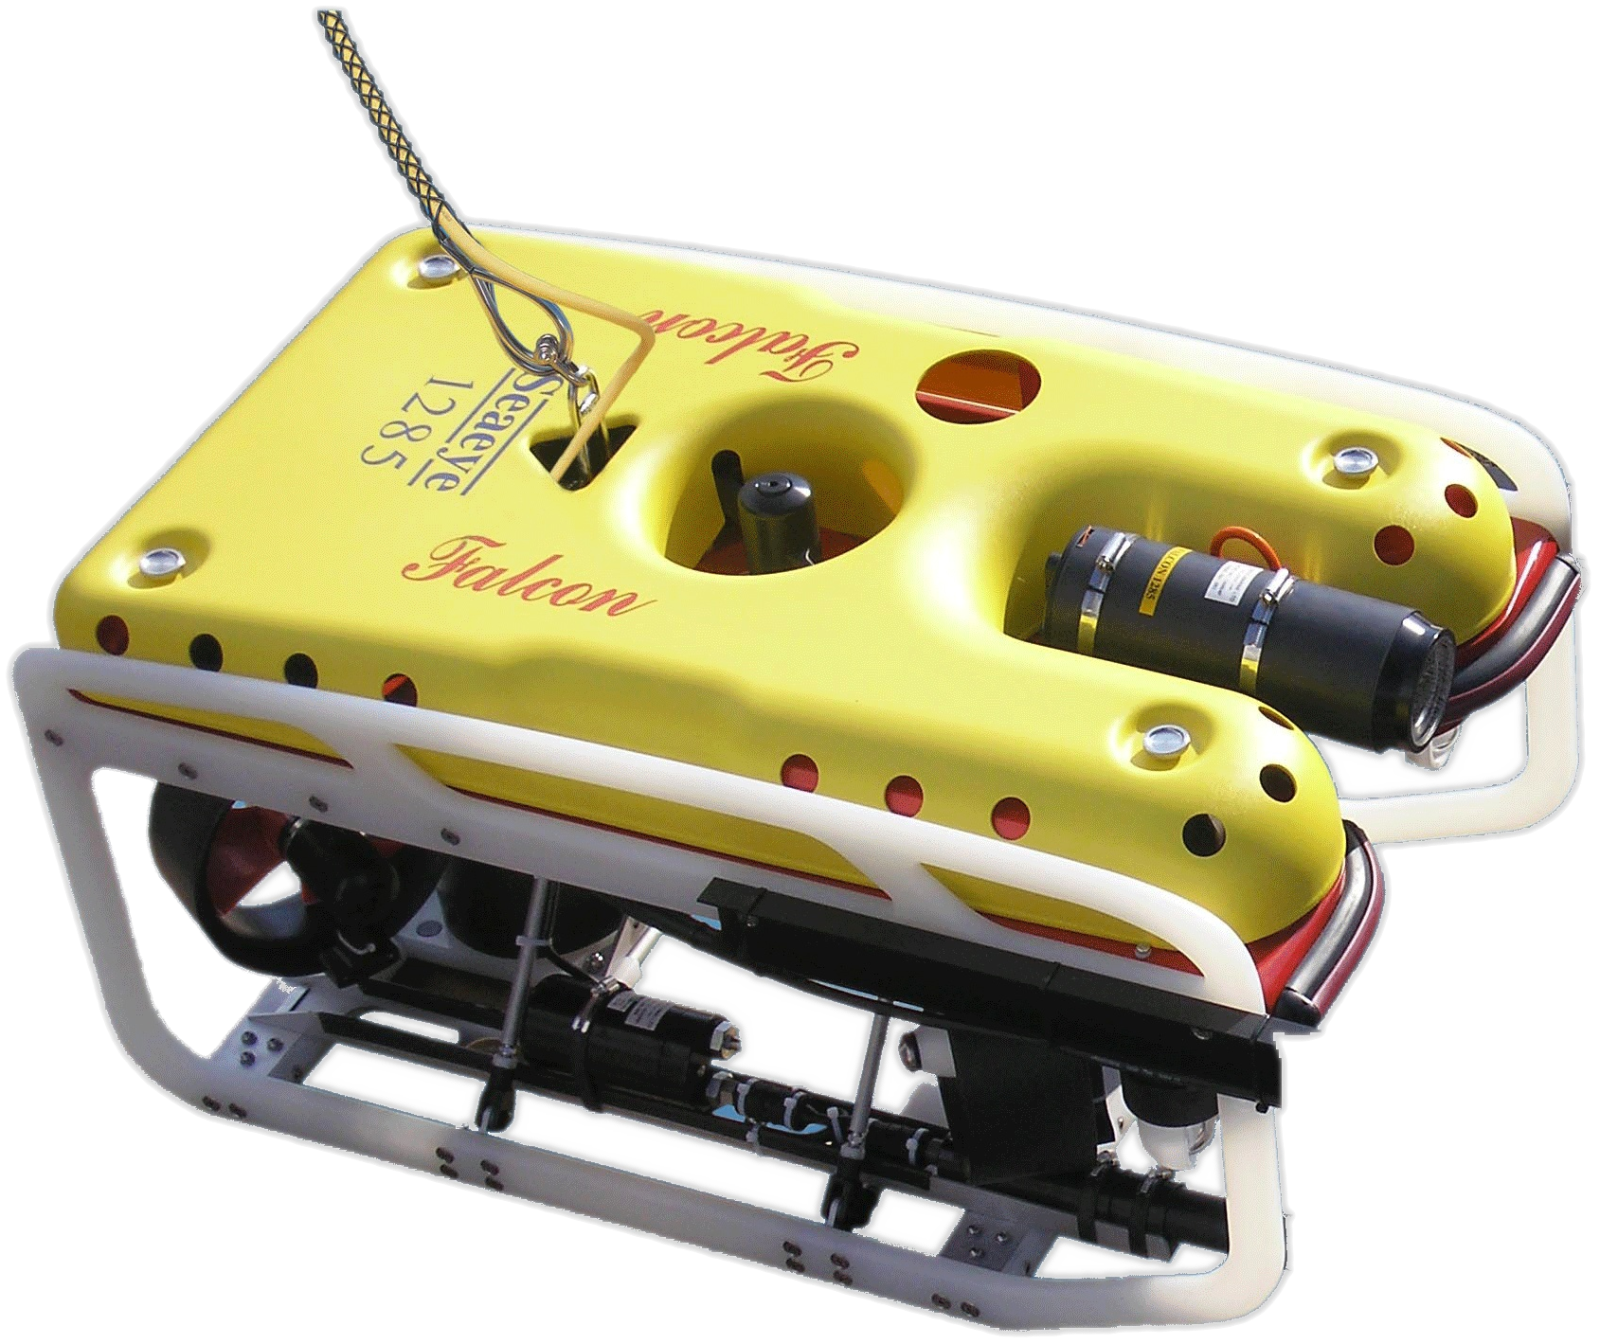
\includegraphics[width=6.2cm]{falcon}
\centering
\caption{Saab SeaEye Falcon}
\label{fig1}%fig:
\end{figure}
Neglecting the elements corresponding to heave, roll and pitch yields\cite{fossen2002marine},
\begin{equation}
\bm{\dot{\eta}}=\textbf{J}(\bm{\eta})\textbf{v}
\end{equation} 
where $\bm{\eta}=[x,y,\psi]^T$ denotes the position and orientation, and $\textbf{v}=[u,v,r]^T$ denotes the velocities.
\begin{equation}
\textbf{J}(\bm{\eta})=\textbf{R}_{z,\psi}=\begin{bmatrix}cos\psi &-sin\psi &0\\sin\psi &cos\psi &0\\0 &0 &1\end{bmatrix}
\end{equation}
\subsection{Dynamics of AUV}
The AUV equations of motion involve statics and dynamics. Statics is concerned with the equilibrium of the vehicle at rest or moving with constant velocity, whereas dynamics is concerned with the vehicle with accelerated motion. The 3 DOF nonlinear dynamic equations of motion can be conveniently expressed as,
\begin{equation}
  \textbf{M}\dot{\textbf{v}}+\textbf{C(v)v}+\textbf{D(v)v}+\textbf{g}(\bm{\eta})=\bm{\tau}
\end{equation}
where $\textbf{M}=diag(M_x,M_y,M_{\psi})$ is the system inertia matrix including the added mass, in general, the damping of AUV can be assumed that the AUV is performing a non-coupled motion, then a approximation damping terms on the diagonal denotes $\textbf{D(v)}=-diag(X_u,Y_v,N_r)-diag(X_{u|u|}|u|,Y_{v|v|}|v|,N_{r|r|}|r|)$, the restoring force $\textbf{g}(\bm{\eta})=0$, while the center of gravity and the center of buoyancy are located vertically on the z-axis.  $\bm{\tau}=[F_u,F_v,F_r]^T$ denotes the thrust force (the control inputs), and $\textbf{C}(\textbf{v})$ denotes the Coriolis-centripetal matrix including added matrix. This simplification is obtained when the origin of body coordinate $(x_b, y_b, z_b)$ coincides with the center gravity of AUV. $$\textbf{C}(\textbf{v})=\begin{bmatrix}0 &0 &-M_yv\\0 &0 &M_xu\\M_yv &-M_xu &0\end{bmatrix}$$

Combining the kinematic equations and the dynamics equations, we estabilish the system model for AUV tracking control problem
\begin{equation}
\dot{\textbf{x}}_e=\begin{bmatrix}
\textbf{J}(\bm{\eta})\textbf{v}\\
\textbf{M}^{-1}(\bm{\tau}-\textbf{C(v)v}-\textbf{D(v)v})
\end{bmatrix}
=f(\textbf{x, u})
\end{equation}
where $\textbf{x}=[x,y,\psi,u,v,r]^T$ denotes the state of the AUV.% and $\bm{\tau}$ denotes the control input.

The AUV system (4) is highly nonlinear. Generally, the linear controller is difficult to solve this problem. In this regard, MPC seems to be an attractive solution which is capable of dealing with nonlinearity of the AUV model.
%For the AUV in 3DOF horizon plane, it is necessary to distribute the generalized control forces $\tau\in \mathbb{R}^n$ to the thrusters. In this paper, we use the open-frame AUV/ROV Saab SeaEye Falcon model\cite{6289904}, so the control inputs can be written as $\textbf{u}=[u_1,u_2,u_3,u_4]^T$. The representation control forces is:
%\begin{equation}
%\bm{\tau}=T(\alpha)\textbf{u}
%\end{equation}
%where $T(\alpha)$ is the control allocation matrix.
\subsection{Problem Formulation}
%1.reference trajectory
%main refer Fossen CH10 and chao \cite{RN33}

Consider a horizontal time-varying reference trajectory 
\begin{equation}
\dot{\textbf{x}}_d(t)=f(x_d(t),u_d(t))
\end{equation}
where $\textbf{x}_d=[x_d,y_d,\psi_d,u_d,v_d,r_d]^T$. The reference trajectory is generated by a virtual reference AUV of the same dynamics, hence
\begin{equation}
\begin{split}
\dot{x}_d&=u_dcos\psi_d-v_dsin\psi_d\\
\dot{y}_d&=u_dsin\psi_d+v_rcos\psi_d\\
\dot{\psi}_d&=r_d
\end{split}
\end{equation}
For the AUV system has a feasible reference, we define the $\textbf{x}_d=[x_d,y_d,\psi_d,u_d,v_d,r_d]^T$ as,
\begin{equation}
\begin{split}
\psi_d(t)&=atan2(\dot{y}_d(t),\dot{x}_d(t))\\
u_d(t)&=\sqrt{\dot{x}_d^2(t)+\dot{y}_d^2(t)}\\
v_d(t)&=0\\
r_d(t)&=(\dot{x}_d(t)\ddot{y}_d(t)-\dot{y}_d(t)\ddot{x}_d(t))/(\dot{x}_d^2(t)+\dot{y}_d^2(t))
\end{split}
\end{equation}
where $atan2$ is the four-quadrant inverse tangent operator.

%3.
\subsection{Lyapunov-based Controller}
Assuming that there exists a Lyapunov-based controller $u(t)=h(x(t))$ which satisfies input constraints on $u$ for all $x$ inside a given stability region and renders the origin of the closed-loop system asymptotically stable. Using the converse Lyapunov theorems, this assumption implies that ehere exist functions $\alpha(\cdot), i=1,2,3,4$ of class $\mathcal{K}$ and a Lyapunov function $V$ for the closed-loop system which is continuous and bounded, that satisfy the following inequalities,
\begin{equation}
\begin{split}
\alpha_1(||x||)\leq V(x)\leq& \alpha_2(||x||)\\
%\frac{\partial V(x)}{\partial x}f(x,h(x),0)\leq \frac{\partial V(x)}{\partial x}f(x,u,0)
\frac{\partial V(x)}{\partial x}f(x,h(x),0)\leq& -\alpha_3(||x||)\\
|\frac{\partial V(x)}{\partial x}|\leq& \alpha_4(||x||)\\
h(x)\in& U
\end{split}
\end{equation}
where $\Omega\subseteq D$ denotes the stability region of the closed-loop system under the control $u=h(x)$, $D$ is an open neighborhood of the origin, $\forall x\subseteq D\in \mathbb{R}^n$.


\section{Main Results}

\subsection{Lyapunov-Based Model Predictive tracking Controller}
Assuming the AUV system is sampled at the time instants $t_k,k=0,1,2,...$, and the sampling period is $\delta$. To faciliate the predictive trajectory of the AUV, we clarify
\begin{itemize}
\item $\textbf{u}^*(s|t_k),s\in[t_k,t_k+T]$ denotes the optimal (i.e., actual) predictive control input of the AUV.
\item $ \hat {\textbf{u}}(s|t_k),s\in[t_k,t_k+T]$ denotes the assumed predictive control input of the AUV.
\end{itemize}

The corresponding state trajectories are labeled in the same way, i.e., $\bm\eta^*$ denotes the optimal predictive trajectory and $\hat{\bm{\eta}}(s|t_k)$ denotes the assumed predictive trajectory.

Consider the time-varying reference trajectory $\textbf{x}_d\in \mathbb{R}^n $, the LMPC can be designed 

\begin{subequations} \label{eq:9}
\begin{align}
\min_{x\in S(\delta)}\quad J=\int_{t_0}^{t_0+T}&(||\hat{\textbf{{x}}}(s)-\textbf{x}_d(s)||_Q+||\textbf{u}(s)||_R)ds\label{eq:a}\\
s.t.\qquad \dot{\textbf{x}}(s)&= f(\hat {\textbf{x}}(s),\hat{\textbf{u}}(s))\label{eq:b}\\
\hat{\textbf{x}}(t_k)&=\textbf{x}(t_k)\label{eq:9c}\\
|\hat{\textbf{u}}(s)|&\leq \textbf{u}_{max}\label{eq:9d}\\
|\Delta\hat{\textbf{u}}(s)|&\leq\Delta \textbf{u}_{max}\label{eq:9e}\\
\frac{\partial V(x)}{\partial \textbf{x}}f(x,u)&\leq \frac{\partial V(x)}{\partial \textbf{x}}f(x,h(x))\label{eq:9f}
\end{align}
\end{subequations}
where $S(\delta)$ is the family of piece-wise constant functions with sampling period $\delta$, $T$ is the prediction horizon, $Q$ and $R$ are positive definite symmetric weighting matrices. 

%From Changxin liu Lyapunov-based tracking control
%the control model
The error dynamics,
\begin{equation}
\dot{\textbf{x}}(t)=f(\textbf{x}_e(t),\textbf{u}_e(t))
\end{equation}

For a fixed prediction horizon N, we consider the cost function for the tracking problem as follows,
\begin{equation}
J(\textbf{x}_e(t_k),\textbf{u}_e(t_k))=\int_{t_k}^{t_k+N}[||\textbf{x}_e(\tau)||_Q^2+||\textbf{u}_e(\tau)||_R^2]d\tau
\end{equation}
where $\textbf{x}_e(\tau)$, $\tau\in [t_k,t_k+N]$ is the predicted state trajectory originating from $\textbf{x}_e(t_k)$ subject to the tracking dynamics and predictd input sequence $\textbf{u}_e(\tau)$. $Q$ and $R$ are positive definite symmetric weight matrixes. MPC optimization problem can be solved online and formulated as follows,
\begin{equation}
\begin{split}
\min\limits_{\textbf{u}_e}&J(\textbf{x}_e(t_k),\textbf{u}_e(t_k))\\
s.t.\quad %&\textbf{x}_e(t_k),\\
 &\textbf{u}_e(t)\in\mathbb{U},\quad t\in[t_k,t_k+N]\\
&\dot{V}(\textbf{x}_e(t_k),\textbf{u}_e(t_k))\leq \dot{V}(\textbf{x}_e(t_k),h(\textbf{x}_e(t_k))\\
&\dot{\textbf{x}}(t)=f(\textbf{x}_e(t),\textbf{u}_e(t)), \quad t\in[t_k,t_k+N]
\end{split}
\end{equation}
where
\begin{equation}
h(\textbf{x}_e)=
\begin{bmatrix}-\xi_2tanh(x_e)\\ 
-\frac{\lambda_1 v_ry_esin(\theta_e)}{(1+x_e^2+y_e^2)\theta_e}-\xi_1 tanh(\theta_e)
\end{bmatrix}
\end{equation}
$h(\textbf{x}_e)$ is a global bounded state feedback tracking controller.
\begin{equation}
V(\textbf{x}_e)=\frac{\lambda_1}{2}log(1+x_e^2+y_e^2)+\frac{1}{2}\theta_e^2
\end{equation}
$V(\textbf{x}_e)$ is the corresponding control Lyapunov function, where $\lambda_1$, $\xi_1$ and $\xi_2$ are positive design parameters. It is assumed that $\mathbb{U}\subset \mathbb{R}^2$ is compact and convex, and $\textbf{0}$ is contained in the interior of $\mathbb{U}$
\subsection{Stability Analysis}
The LMPC 
\section{Simulation Study}
In the simulation, the results of the trajectory tracking control of the AUV under input constraints are presented. The simulation experiments are carried by using the dynamic model of Falcon\cite{proctor2014semi}. 
\subsection{Parameter selection}
\textbf{Case 1:}
The first reference trajectory in the simulation is a sinusoidal shape trajectory defined as follows,
\begin{equation} 
\begin{split}
   x_d=0.5t&\\
   y_d=sin(0.5t)&
\end{split}
\end{equation}

\textbf{Case 2:}
The second reference trajectory is an eight-shape trajectory defined as,
\begin{equation}
\begin{split}
   x_d=sin(0.5t)&\\
   y_d=sin(0.25t)&
\end{split}
\end{equation}
The parameters of LMPC are designed as follows, the sampling period $\delta=0.2s$ the predictive horizon is $T=1.4s$. In the cost function, as in \cite{shen1lyapunov} the weighting matrices are chosen as $Q=diag(10^5,10^5,10^3,10^2,\\10^2,10^2)$, $R=diag(10^{-4},10^{-4},10^{-4},10^{-4}$ and $P=diag(10^3,10^3,10^2,10,10,10)$. In $\textbf{Case1}$ the initial condition is $(0,-0.5,\pi/2,0,0,0)$, and in $\textbf{Case2}$ the initial condition is $(-1,0,0,0,0,0)$. 
\subsection{Tracking Performance}
The simulation is carried out by using the MATLAB package and the optimization algorithm is executed by the fminicon function. The simulation results are presented through Fig.2 to Fig.7. The black curve is the reference trajectory, and the red one is the AUV trajectory with the LMPC in Fig.2 and Fig.5.

\graphicspath{{./Fig/}}
\begin{figure}
\vspace{-7cm}
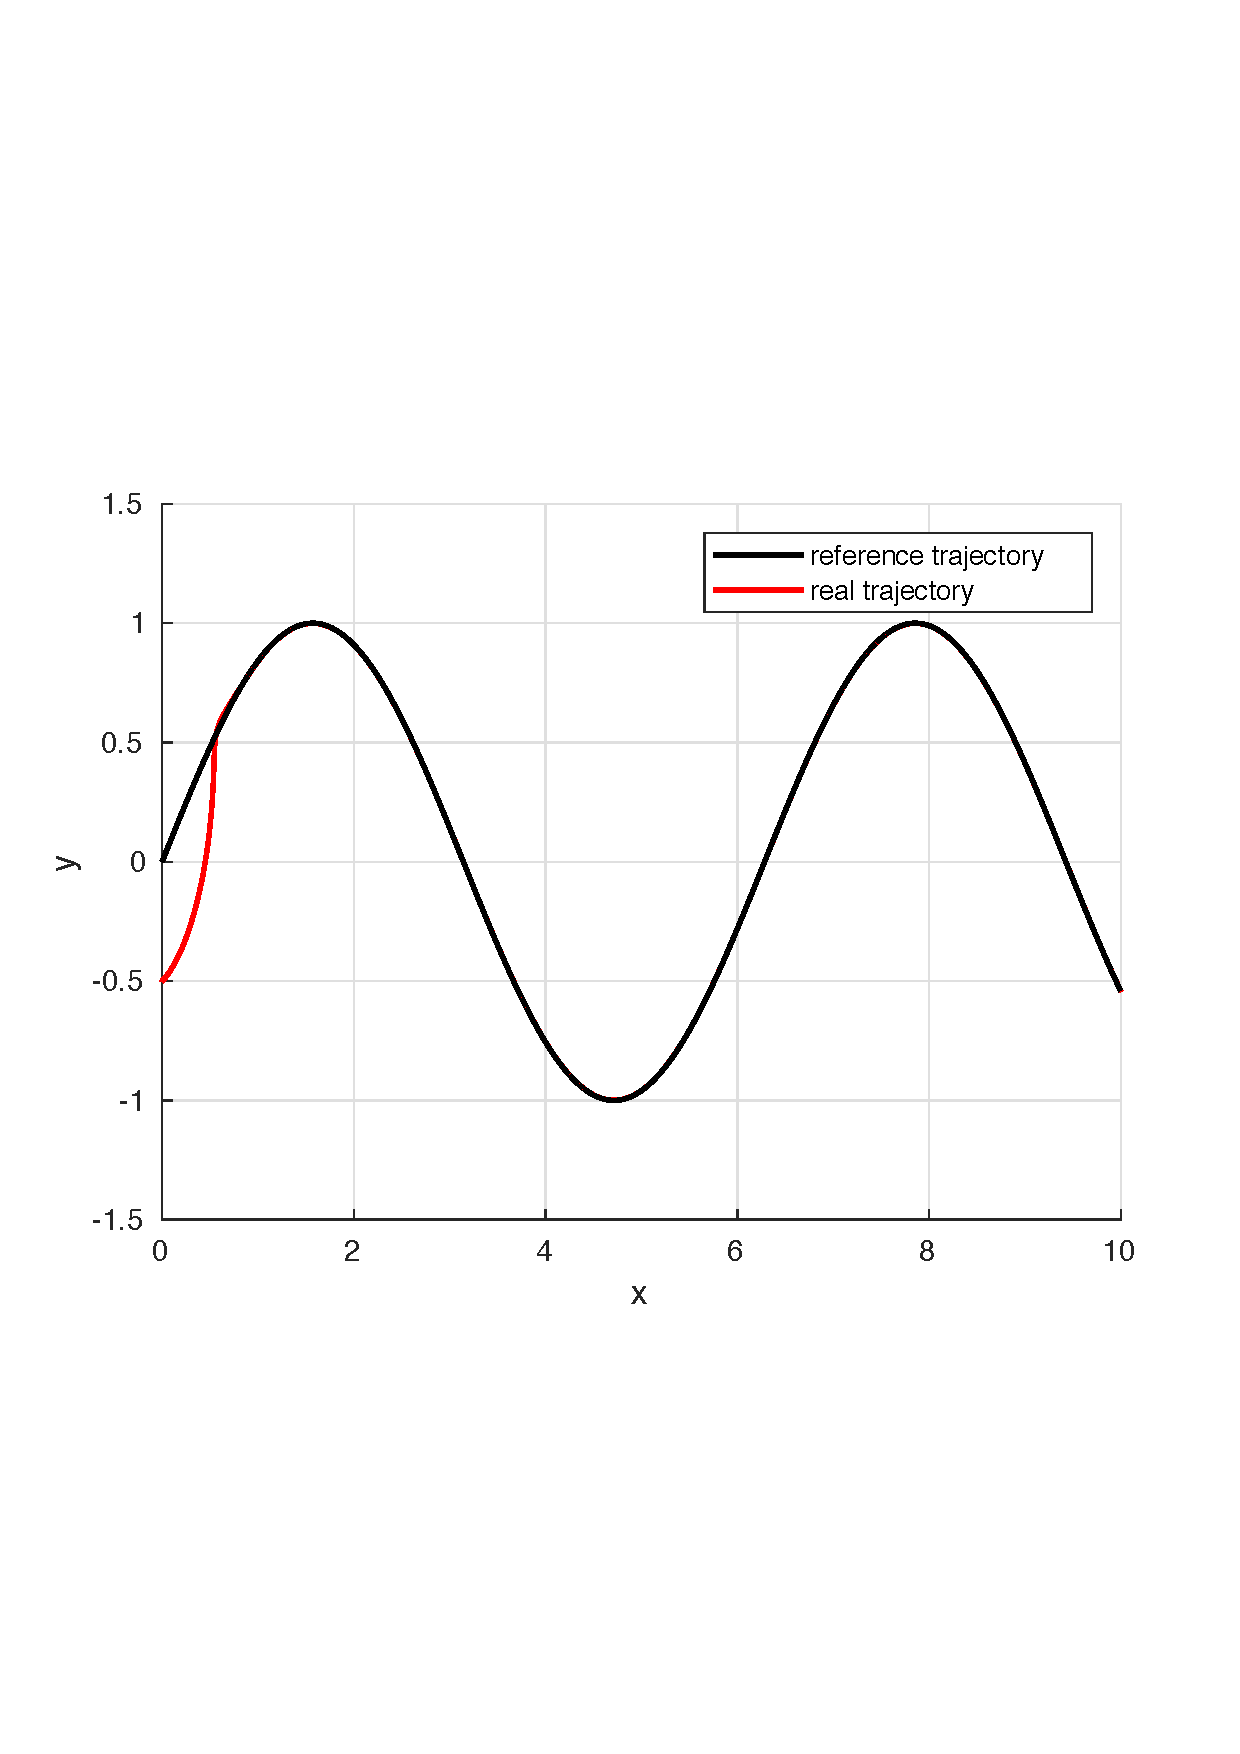
\includegraphics[scale=0.8]{tracking2.pdf}
%\centering
\vspace{-7cm}
\caption{The AUV trajectory in X-Y plane}
\label{fig:fig2}%
\end{figure}

\graphicspath{{./Fig/}}
\begin{figure}
\vspace{-7cm}
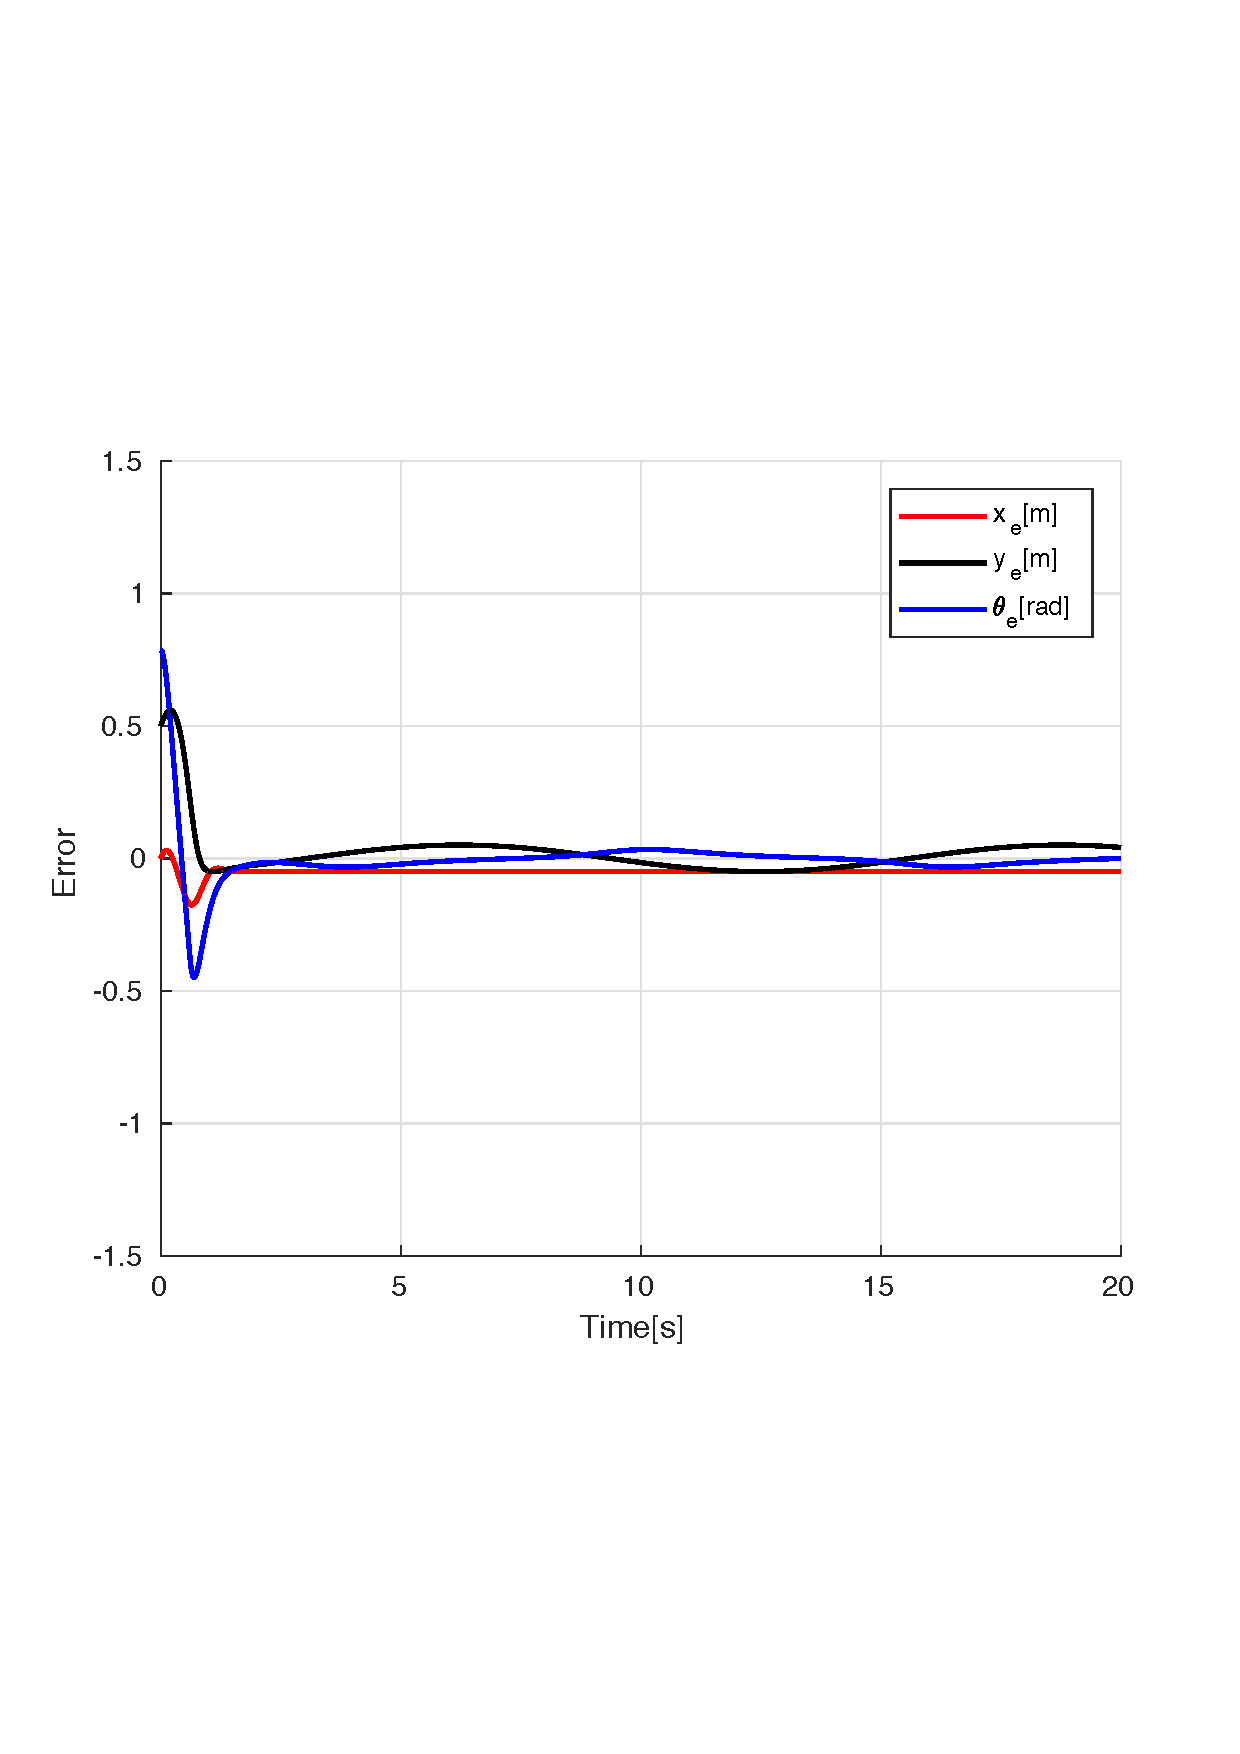
\includegraphics[scale=0.8]{error2.pdf}
\vspace{-5cm}
\centering
\caption{The tracking error}
\label{fig:fig3}%
\end{figure}


\graphicspath{{./Fig/}}
\begin{figure}
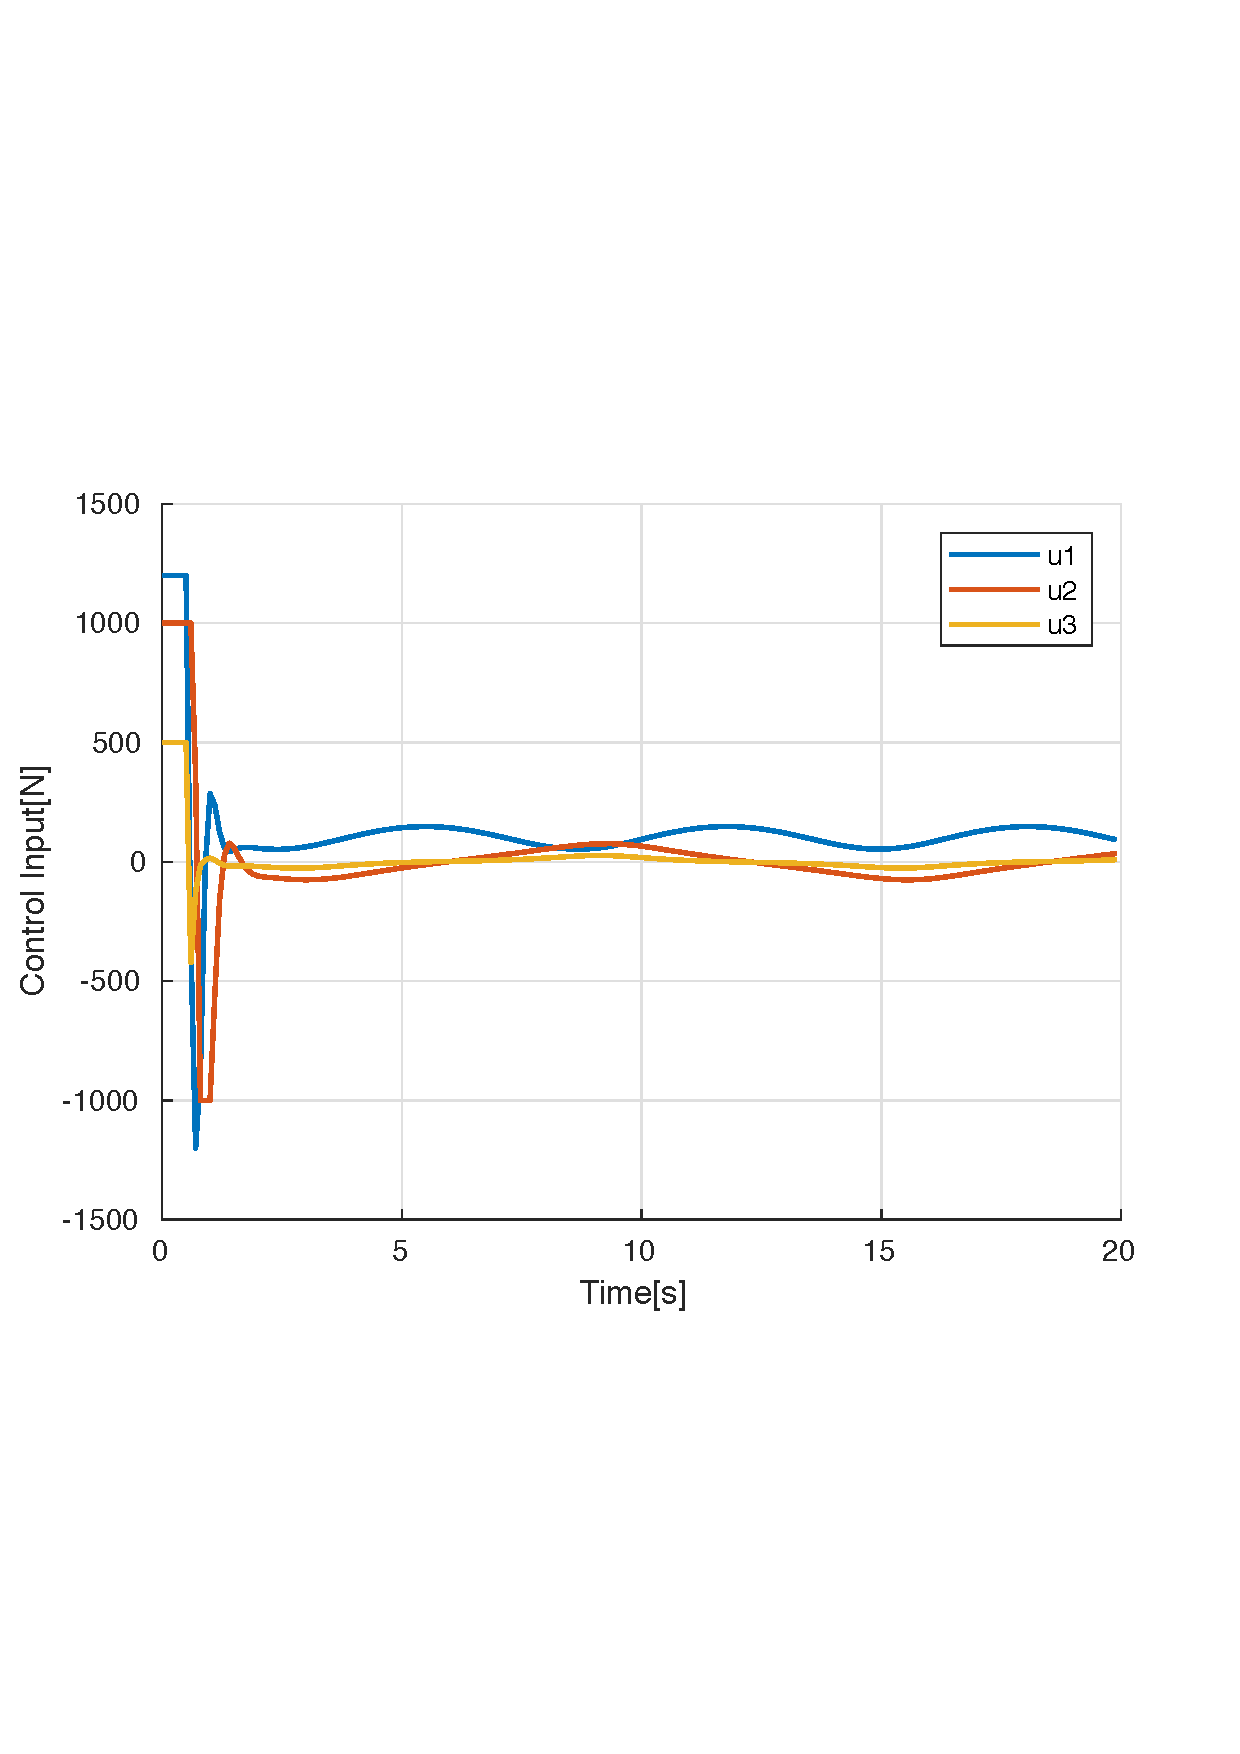
\includegraphics[scale=0.5]{input2.pdf}
\centering
\caption{The control input signal}
\label{fig:fig4}%fig:
\end{figure}

\graphicspath{{./Fig/}}
\begin{figure}
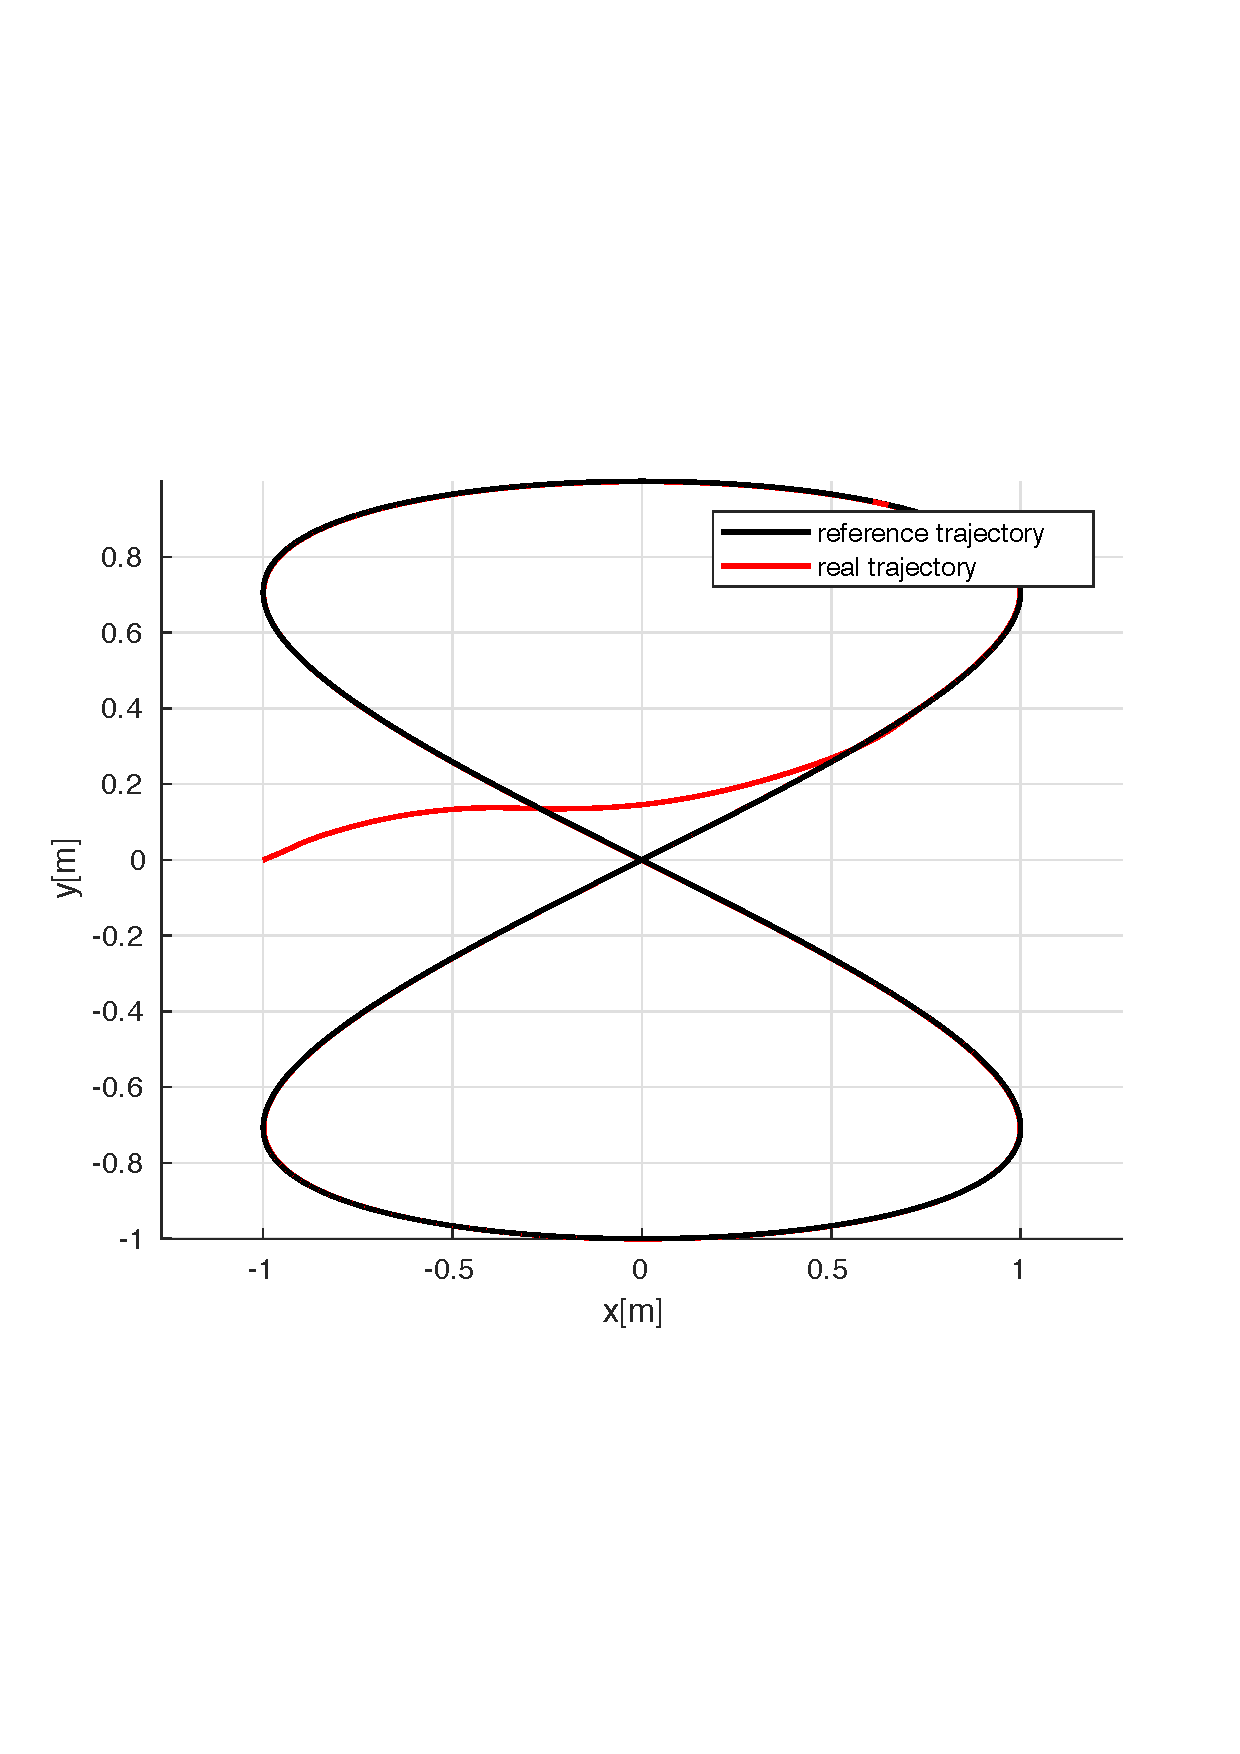
\includegraphics[scale=0.5]{tracking.pdf}
\centering
\caption{The AUV trajectory in X-Y plane}
\label{fig:fig5}%
\end{figure}

\graphicspath{{./Fig/}}
\begin{figure}
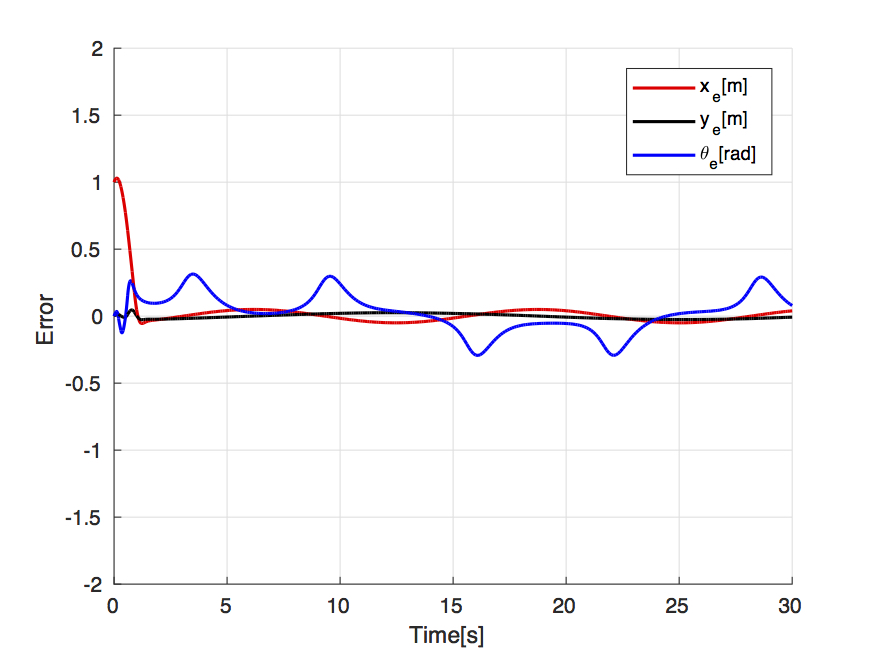
\includegraphics[scale=0.5]{error.jpg}
\centering
\caption{The tracking error}
\label{fig:fig6}%fig:
\end{figure}


\graphicspath{{./Fig/}}
\begin{figure}
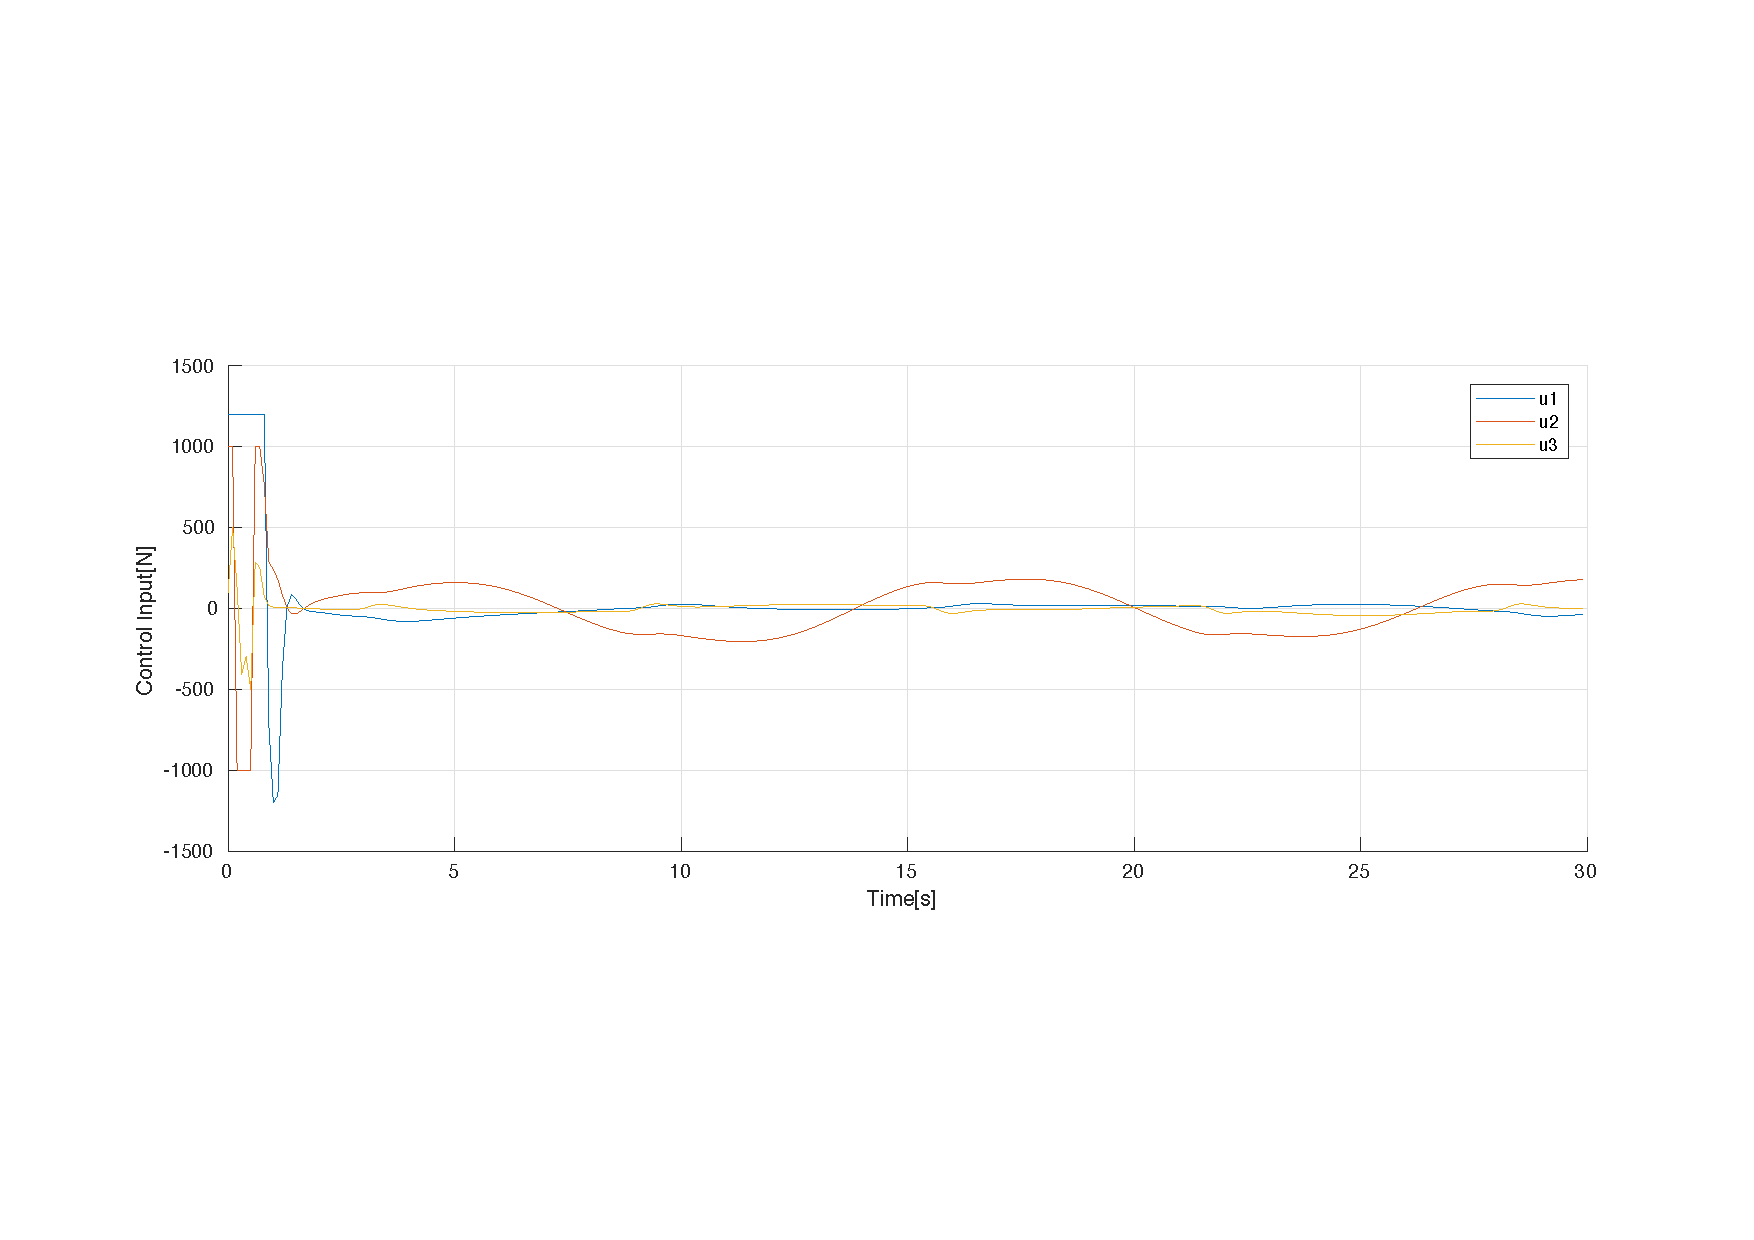
\includegraphics[scale=0.6]{input.pdf}
\centering
\caption{The control input signal}
\label{fig:fig7}%fig:
\end{figure}

\section{Conclusion}
In this work, a LMPC tracking controller was proposed for the AUV subject to input constraints. In order to provide guaranteed stability, the constraints that define the LMPC optimization problems as well as the implementation procedures have to be modified to account for input constraints. The presented LMPC posses an explicit characterization of the closed-loop system stability regions. The simulation results show that the AUV can track the time-varying reference trajectory using the LMPC controller.

\bibliographystyle{IEEEtran}
\bibliography{mpc_tracking}
\end{document}
